\chapter{LTE KPI Forecasting Engine}
\label{ch:forecasting}

\section{Introduction \& Motivation}
\label{sec:forecasting_intro}

Modern LTE network operations have traditionally relied on reactive maintenance paradigms, wherein performance degradation is addressed only after subscriber-facing quality-of-service (QoS) incidents have already occurred. This post-facto approach incurs tangible costs in terms of churn, regulatory penalties, and emergency truck rolls. A paradigm shift toward \emph{proactive maintenance} requires the ability to anticipate Key Performance Indicator (KPI) trajectories before they breach contractual thresholds.

This chapter presents the \textbf{KPI Forecasting \& Predictive Analytics Module}, a cell-level, multi-horizon forecasting engine designed to predict LTE KPI values seven days into the future. The module is architected around three complementary modeling strategies: (i) naive statistical baselines that serve as sanity checks, (ii) classical Holt-Winters exponential smoothing to capture dominant seasonal patterns, and (iii) a gradient-boosted tree regressor (XGBoost) that leverages cross-KPI lag features to model non-linear, multi-variate temporal dependencies. A unified evaluation framework compares all candidates against hold-out data and automatically recommends the most reliable predictor on a per-cell, per-KPI basis.

The remainder of this chapter is organized as follows. Section~\ref{sec:forecasting_theory} reviews the theoretical foundations of time-series forecasting, exponential smoothing, and residual diagnostics. Section~\ref{sec:forecasting_design} defines the module's functional requirements and its interfaces with the degradation analyzer (Chapter~4) and the action analyzer (Chapter~6). Section~\ref{sec:forecasting_data} details the data pipeline, seasonality detection, and leakage-safe feature engineering. Section~\ref{sec:forecasting_models} derives the three forecasting models and the fallback selection logic. Section~\ref{sec:forecasting_eval} establishes the evaluation protocol, residual diagnostics, and feature-importance interpretation. Section~\ref{sec:forecasting_summary} concludes with key findings.


\section{Theoretical Background}
\label{sec:forecasting_theory}

\subsection{Time-Series Forecasting in Telecom Networks}

A univariate time series $\{y_t\}_{t=1}^{T}$ observed for a single cell-KPI pair can be decomposed into four additive components:
\begin{equation}
y_t = T_t + S_t + C_t + \varepsilon_t,
\end{equation}
where $T_t$ denotes the long-term trend, $S_t$ the seasonal oscillation (e.g., weekly traffic cycles), $C_t$ cyclical variations, and $\varepsilon_t$ an irregular residual. In cellular networks, $S_t$ typically dominates because human mobility and usage patterns exhibit strong daily and weekly periodicities. Cyclical components are often negligible at the 30-day observation windows typical of operational dashboards, leaving the forecaster to model $T_t + S_t$ while ensuring that $\varepsilon_t$ is approximately white noise.

Telecom KPIs pose distinct challenges: they are often non-stationary (mean and variance shift with network upgrades or load spikes), heteroscedastic (variance scales with traffic volume), and subject to abrupt structural breaks (hardware failures, neighbor-cell interference). These properties motivate a multi-model strategy rather than reliance on a single inductive bias.

\subsection{Holt-Winters Exponential Smoothing}

Holt-Winters extends simple exponential smoothing by explicitly modeling level, trend, and seasonality. For a series with period $m$, the additive formulation updates three smoothed states:
\begin{align}
\ell_t &= \alpha\left(y_t - s_{t-m}\right) + (1-\alpha)\left(\ell_{t-1} + b_{t-1}\right), \\
b_t &= \beta\left(\ell_t - \ell_{t-1}\right) + (1-\beta)b_{t-1}, \\
s_t &= \gamma\left(y_t - \ell_t\right) + (1-\gamma)s_{t-m},
\end{align}
where $\ell_t$ is the smoothed level, $b_t$ the trend, $s_t$ the seasonal component, and $\alpha, \beta, \gamma \in (0,1)$ are smoothing parameters optimized via maximum likelihood. A multiplicative variant replaces additive seasonality with ratio-based updates when seasonal amplitude scales with the level. In this module, both trend and seasonal component types are configurable (additive, multiplicative, or disabled), allowing the model to adapt to KPIs with weak or strong seasonality.

\subsection{Gradient Boosting for Time-Series (XGBoost)}

While XGBoost is not inherently a sequential model, it can be adapted to time-series forecasting through careful feature engineering that encodes temporal structure into a tabular regression task. Given a target KPI $y_t$, the model learns a mapping
\begin{equation}
\hat{y}_t = f\bigl(\mathbf{x}_t\bigr) + \varepsilon_t,
\end{equation}
where the feature vector $\mathbf{x}_t$ comprises lagged values, rolling statistics, and cross-KPI covariates, all strictly constructed from observations at times $< t$ to prevent data leakage. XGBoost approximates $f$ via an ensemble of $K$ regression trees:
\begin{equation}
\hat{y}_t = \sum_{k=1}^{K} \eta \cdot h_k(\mathbf{x}_t),
\end{equation}
with learning rate $\eta$ and where each $h_k$ is fitted to the negative gradient (pseudo-residuals) of a differentiable loss function. Regularization terms
\begin{equation}
\Omega(h_k) = \gamma T + \tfrac{1}{2}\lambda \sum_{j=1}^{T} w_j^2 + \alpha \sum_{j=1}^{T} |w_j|
\end{equation}
penalize tree complexity ($T$ leaves), leaf weights $w_j$, and enforce sparsity via $L_1$ ($\alpha$) and $L_2$ ($\lambda$) coefficients. These controls are essential given the limited sample size ($\sim$30 days) relative to the engineered feature dimensionality.

\subsection{Residual Diagnostics \& Model Validation}

A well-specified forecasting model should extract all systematic information from the series, leaving residuals that resemble white noise. Two standard tests are employed:

\textbf{Durbin-Watson statistic.} For residuals $\{e_t\}$, the statistic
\begin{equation}
DW = \frac{\sum_{t=2}^{T}(e_t - e_{t-1})^2}{\sum_{t=1}^{T}e_t^2}
\end{equation}
tests for first-order autocorrelation. Values near 2 indicate no autocorrelation; values below 1.5 or above 2.5 suggest positive or negative serial correlation, respectively, implying the model has missed a temporal pattern.

\textbf{Ljung-Box test.} A portmanteau test evaluating the null hypothesis that the first $h$ autocorrelations are jointly zero:
\begin{equation}
Q = T(T+2)\sum_{k=1}^{h}\frac{\hat{\rho}_k^2}{T-k},
\end{equation}
where $\hat{\rho}_k$ is the sample autocorrelation at lag $k$. Under the null, $Q \sim \chi^2(h)$. A $p$-value exceeding 0.05 supports the white-noise hypothesis.

In addition, the Autocorrelation Function (ACF) of residuals is inspected visually; significant spikes outside the 95\% confidence band ($\pm 1.96/\sqrt{T}$) at non-zero lags indicate unmodeled seasonality or trend.


\section{System Requirements \& Design}
\label{sec:forecasting_design}

\subsection{Functional Requirements}

The forecasting module satisfies the following functional requirements derived from the broader proactive maintenance pipeline:

\begin{enumerate}[FR-1.]
    \item \textbf{Multi-model execution:} Support at least one statistical benchmark (Holt-Winters), one machine-learning model (XGBoost), and naive baselines.
    \item \textbf{Leakage-safe feature engineering:} All predictive features must be computable using only past observations relative to the forecast origin.
    \item \textbf{Automatic model selection:} Compare each candidate against a naive baseline on a hold-out window and recommend the best performer.
    \item \textbf{Seasonality quantification:} Compute a seasonality-strength score per cell-KPI pair to inform model selection and UI ranking.
    \item \textbf{Residual diagnostics:} Report Durbin-Watson, Ljung-Box, and ACF plots for every XGBoost run.
    \item \textbf{Recursive multi-step forecasting:} Generate a 7-day ahead trajectory by iteratively appending predictions to history and re-deriving features.
    \item \textbf{LLM-ready export:} Emit a structured textual summary of forecasts, trends, and alerts for downstream natural-language reasoning modules.
\end{enumerate}

\subsection{Module Architecture \& Data Flow}

Figure~\ref{fig:architecture} illustrates the internal data flow. The uploaded CSV passes through a loader that coerces percentages and renames raw counters to canonical short names. The seasonality analyzer then decomposes each cell-KPI series via STL and computes a strength score. The feature engineer constructs a leakage-safe design matrix, which is split into training and hold-out sets. The forecasting engine trains all candidate models, evaluates them on the hold-out window, and triggers residual diagnostics for XGBoost. Finally, a report generator assembles an LLM-ready prompt summarizing the results.

\begin{figure}[htbp]
    \centering
    \begin{tikzpicture}[
        node distance=1.4cm and 2.2cm,
        box/.style={rectangle, draw, rounded corners, minimum width=2.8cm, minimum height=0.9cm, align=center, font=\small},
        arrow/.style={->, >=stealth, thick}
    ]
        \node[box, fill=gray!10] (csv) {Cleaned KPI CSV};
        \node[box, right=of csv, fill=blue!5] (load) {Data Loader};
        \node[box, right=of load, fill=orange!5] (seas) {Seasonality\\Analyzer};
        \node[box, below=of seas, fill=green!5] (feat) {Feature\\Engineer};
        \node[box, left=of feat, fill=red!5] (model) {Forecasting\\Engine};
        \node[box, left=of model, fill=purple!5] (diag) {Residual\\Diagnostics};
        \node[box, below=of diag, fill=cyan!5] (report) {LLM Report\\Generator};

        \draw[arrow] (csv) -- (load);
        \draw[arrow] (load) -- (seas);
        \draw[arrow] (seas) -- (feat);
        \draw[arrow] (feat) -- (model);
        \draw[arrow] (model) -- (diag);
        \draw[arrow] (diag) -- (report);
        \draw[arrow, dashed] (model.south) -- ++(0,-0.5) -| (report.north);
        \draw[arrow, dashed] (seas.east) -- ++(0.8,0) |- (model.east);
    \end{tikzpicture}
    \caption{High-level data-flow diagram of the KPI Forecasting Module. Solid arrows indicate primary data flow; dashed arrows indicate metadata or control signals.}
    \label{fig:architecture}
\end{figure}

\subsection{Interface with Adjacent Modules}

The forecasting module occupies a central position in the proactive maintenance pipeline:

\begin{itemize}
    \item \textbf{Upstream (Chapter~4 -- Degradation Analyzer):} The degradation analyzer flags anomalous cells and KPIs exhibiting recent downward trends or threshold breaches. These flagged entities are prioritized in the forecasting UI, ensuring that operator attention and computational resources are directed toward the most critical network elements.

    \item \textbf{Downstream (Chapter~6 -- Action Analyzer):} The 7-day ahead forecasts produced by this module serve as primary inputs to the action analyzer. Predicted traffic spikes, for example, trigger preemptive capacity scaling recommendations, while forecasted drops in handover success rates may prompt neighbor-list audits before subscriber impact materializes.

    \item \textbf{Lateral (Chapter~7 -- Telecom RAG Assistant):} The LLM-ready report generator outputs structured prompts that the Retrieval-Augmented Generation (RAG) assistant consumes to produce natural-language root-cause hypotheses and remediation strategies.
\end{itemize}


\section{Data Pipeline \& Preprocessing}
\label{sec:forecasting_data}

\subsection{Input Data Format}

The module ingests a cleaned CSV export containing daily cell-level observations. Each row corresponds to a single cell-date pair, with columns mapped from raw counter names to canonical short identifiers. Table~\ref{tab:kpis} enumerates the supported KPIs grouped by the standard 3GPP performance pillar.

\begin{table}[htbp]
    \centering
    \caption{Supported LTE KPIs with canonical internal names and performance categories.}
    \label{tab:kpis}
    \begin{tabular}{@{}lll@{}}
        \toprule
        \textbf{Category} & \textbf{Display Name} & \textbf{Internal Name} \\
        \midrule
        Traffic & DL Traffic Volume (GBytes) & \texttt{DL\_Traffic} \\
        Traffic & DL Average Throughput (Mbps) & \texttt{DL\_Throughput} \\
        Traffic & Average UE Number & \texttt{Avg\_UE\_Number} \\
        Traffic & Active Users & \texttt{Active\_Users} \\
        Accessibility & RRC Setup Success Rate (\%) & \texttt{RRC\_Setup\_SR} \\
        Retainability & E-RAB Drop Rate (\%) & \texttt{ERAB\_Drop\_Rate} \\
        Mobility & Intra-Freq HO Success Rate (\%) & \texttt{Intra\_HO\_SR} \\
        Mobility & Inter-Freq HO Success Rate (\%) & \texttt{Inter\_HO\_SR} \\
        Integrity & DL Average CQI & \texttt{DL\_CQI} \\
        Integrity & DL IBLER (\%) & \texttt{DL\_IBLER} \\
        Utilization & DL PRB Utilization (\%) & \texttt{DL\_PRB\_Util} \\
        Experience & User DL Avg Throughput (Mbps) & \texttt{User\_DL\_Throughput} \\
        \bottomrule
    \end{tabular}
\end{table}

Percentage and rate columns are coerced from string representations (e.g., ``98.5\%'') to floating-point values during ingestion to ensure numeric compatibility across the pipeline.

\subsection{Seasonality Detection}

Before model training, each cell-KPI series is decomposed using Seasonal and Trend decomposition using Loess (STL). The decomposition separates the observed series into trend, seasonal, and residual components. To quantify the prominence of the seasonal pattern, the seasonality strength score proposed by Hyndman and Athanasopoulos is computed:
\begin{equation}
F_{\text{seasonal}} = \max\left(0,\; 1 - \frac{\text{Var}(R_t)}{\text{Var}(S_t + R_t)}\right),
\label{eq:seasonality_strength}
\end{equation}
where $S_t$ is the seasonal component and $R_t$ the residual. A score approaching 1.0 indicates that most variation is explained by seasonality, whereas a score near 0.0 implies a weak or noisy seasonal signal. This score is used to sort the cell-selection dropdown (strongest seasonality first) and to display contextual warnings when lag-7 or weekly-mean features may be unreliable.

\subsection{Cross-KPI Feature Engineering}

A leakage-safe feature matrix is constructed for each target KPI by drawing exclusively from past observations. Table~\ref{tab:features} categorizes the engineered features and their operational rationale.

\begin{table}[htbp]
    \centering
    \caption{Leakage-safe feature engineering taxonomy for the XGBoost regressor.}
    \label{tab:features}
    \begin{tabular}{@{}p{3.2cm}p{4.8cm}p{5.5cm}@{}}
        \toprule
        \textbf{Feature Category} & \textbf{Examples} & \textbf{Rationale} \\
        \midrule
        Lag features & \texttt{lag\_1} $\ldots$ \texttt{lag\_7}, \texttt{lag\_14}, \texttt{lag\_21} & Capture recent historical levels and weekly periodicity. \\
        Rolling statistics & \texttt{rolling\_mean\_7}, \texttt{rolling\_std\_7}, \texttt{rolling\_mean\_3}, \texttt{rolling\_mean\_14}, \texttt{rolling\_mean\_21} & Smooth local trends and characterize volatility over multiple horizons. \\
        Normalized lags & \texttt{lag7\_norm} = \texttt{lag\_7} / \texttt{rolling\_mean\_7} & Express deviation relative to the recent weekly average. \\
        Momentum & \texttt{momentum\_1} = \texttt{lag\_1} $-$ \texttt{lag\_2}, \texttt{momentum\_2} = \texttt{lag\_2} $-$ \texttt{lag\_3} & Encode rate of change and local acceleration. \\
        Week-over-week diff & \texttt{wow\_diff} = \texttt{lag\_1} $-$ \texttt{lag\_8} & Isolate week-to-week drift. \\
        Shape descriptors & \texttt{weekly\_slope} = \texttt{lag\_1} $-$ \texttt{lag\_7} & Capture intra-week trajectory. \\
        Cross-KPI lags & \texttt{ERAB\_Drop\_Rate\_lag1}, \texttt{Inter\_HO\_SR\_lag1} & Leverage inter-KPI correlations (e.g., throughput vs.~PRB utilization). \\
        Lag interactions & \texttt{lag1\_x\_lag7} = \texttt{lag\_1} $\times$ \texttt{lag\_7} & Model non-linear interactions between recent and weekly history. \\
        \bottomrule
    \end{tabular}
\end{table}

Notably, NaN values arising from insufficient history (e.g., \texttt{lag\_21} on day 5) are intentionally preserved rather than imputed. XGBoost handles missing values natively via its split-based decision logic, learning optimal directions for absent features without introducing synthetic bias.


\section{Forecasting Models}
\label{sec:forecasting_models}

\subsection{Baseline Models}

Two naive strategies provide lower-bound benchmarks against which any sophisticated model must justify its complexity:

\begin{enumerate}
    \item \textbf{Naive (last-value) baseline:} $\hat{y}_{T+h} = y_T$ for all $h \in \{1,\ldots,7\}$. This assumes the most recent observation is the best predictor of the immediate future.
    \item \textbf{Weekly-mean baseline:} If at least seven historical observations exist, $\hat{y}_{T+h} = \frac{1}{7}\sum_{i=0}^{6} y_{T-i}$. This captures a crude local average and is particularly competitive when the series is stable.
\end{enumerate}

The baseline with the lowest Mean Absolute Error (MAE) on the hold-out window is designated the ``best baseline.'' If a candidate model fails to outperform this baseline, the system flags the cell as one where added model complexity does not translate to predictive value.

\subsection{Holt-Winters Exponential Smoothing}

The Holt-Winters implementation uses \texttt{statsmodels.tsa.holtwinters.ExponentialSmoothing}. Both trend and seasonal components are configurable via the user interface: trend $\in \{\text{add}, \text{mul}, \text{None}\}$ and seasonality $\in \{\text{add}, \text{mul}, \text{None}\}$, with the seasonal period defaulting to 7 days to match weekly usage cycles. The model is fit via maximum-likelihood optimization of the smoothing parameters and then used to generate both in-sample fitted values and out-of-sample forecasts for the hold-out window and the future 7-day horizon.

Holt-Winters serves as the classical counterpart to XGBoost: it excels when the series exhibits a clear, stable seasonal structure and requires no manual feature engineering. Its primary limitation is the assumption that seasonality is regular and that trend behavior does not shift abruptly---conditions that are occasionally violated in cellular networks during special events or hardware upgrades.

\subsection{XGBoost Regressor with Recursive Multi-Step Forecasting}

The XGBoost model is trained on the feature matrix described in Section~\ref{sec:forecasting_data} using a configurable hold-out window (default: the most recent 4 days). Hyperparameters exposed through the interface include:

\begin{itemize}
    \item \texttt{n\_estimators} $\in [50, 300]$, default 100
    \item \texttt{learning\_rate} $\in \{0.01, 0.03, 0.05, 0.1, 0.2\}$, default 0.05
    \item \texttt{max\_depth} $\in [2, 6]$, default 3
    \item \texttt{subsample} $\in [0.5, 1.0]$, default 0.8
\end{itemize}

Fixed regularization constants are \texttt{colsample\_bytree}=0.8, \texttt{min\_child\_weight}=3, \texttt{reg\_alpha}=0.1, and \texttt{reg\_lambda}=1.0, chosen to combat overfitting given the limited temporal depth of the dataset.

For multi-step forecasting, a recursive strategy is employed. Rather than training seven separate one-step models, a single regressor is retrained on the full available history and then iteratively forecasts one day at a time:

\begin{algorithm}[H]
    \caption{Recursive 7-Day Ahead Forecast}
    \label{alg:recursive}
    \begin{algorithmic}[1]
        \Require Full history $\mathcal{H} = \{y_1, \ldots, y_T\}$, feature builder $\phi(\cdot)$, trained model $f$
        \State $\mathcal{H}^{(0)} \gets \mathcal{H}$
        \For{$h = 1$ \textbf{to} $7$}
            \State $\mathbf{x}_{T+h} \gets \phi\bigl(\mathcal{H}^{(h-1)}\bigr)$
            \State $\hat{y}_{T+h} \gets f(\mathbf{x}_{T+h})$
            \State Append $\hat{y}_{T+h}$ to $\mathcal{H}^{(h-1)}$ to form $\mathcal{H}^{(h)}$
        \EndFor
        \State \Return $\{\hat{y}_{T+1}, \ldots, \hat{y}_{T+7}\}$
    \end{algorithmic}
\end{algorithm}

This approach preserves cross-feature and cross-KPI relationships at each step but accumulates prediction error as the horizon extends. The 7-day window was selected to balance operational relevance (typical maintenance scheduling cadence) with forecast fidelity.

\subsection{Model Selection \& Fallback Logic}

After all candidates are evaluated on the hold-out window, the system applies the following selection protocol:

\begin{enumerate}
    \item Compute MAE for XGBoost, Holt-Winters, and the best baseline.
    \item Identify the model with the lowest MAE.
    \item If the best baseline outperforms both XGBoost and Holt-Winters, emit a \emph{fallback recommendation}: ``Model is not adding real value for this cell; use baseline.''
    \item Otherwise, promote the winning model and display its metrics alongside the baseline for transparency.
\end{enumerate}

This protocol ensures that the system does not overstate the value of machine learning when the underlying series is inherently unpredictable or stable. Figure~\ref{fig:metrics_panel} shows the UI presentation of this comparison.

\begin{figure}[htbp]
    \centering
    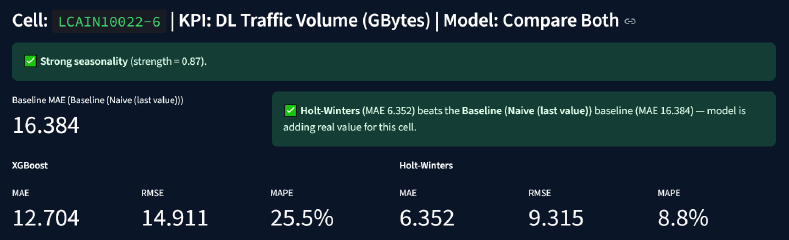
\includegraphics[width=0.95\textwidth]{figures/chapter05/image3.png}
    \caption{Dashboard header for cell \texttt{LCAIN10022-6} forecasting DL Traffic Volume. The seasonality strength badge (0.87) and baseline comparison panel confirm that Holt-Winters (MAE 6.352) substantially outperforms the naive baseline (MAE 16.384), validating model deployment for this cell.}
    \label{fig:metrics_panel}
\end{figure}


\section{Model Evaluation \& Diagnostics}
\label{sec:forecasting_eval}

\subsection{Accuracy Metrics}

Three standard metrics quantify hold-out predictive accuracy:

\begin{align}
\text{MAE} &= \frac{1}{H}\sum_{h=1}^{H} \bigl|y_{T+h} - \hat{y}_{T+h}\bigr|, \\
\text{RMSE} &= \sqrt{\frac{1}{H}\sum_{h=1}^{H} \bigl(y_{T+h} - \hat{y}_{T+h}\bigr)^2}, \\
\text{MAPE} &= \frac{100\%}{H}\sum_{h=1}^{H} \left|\frac{y_{T+h} - \hat{y}_{T+h}}{y_{T+h}}\right|.
\end{align}

MAE is robust to outliers and directly interpretable in the original KPI units (e.g., GBytes). RMSE penalizes large deviations more heavily, making it sensitive to occasional miss-predictions during anomalous days. MAPE provides a scale-independent percentage error but is undefined for zero-valued observations and unstable for series near zero; it is reported primarily for relative comparison across KPIs with different magnitudes.

\subsection{Baseline Comparison}

Figure~\ref{fig:forecast_chart} presents a representative forecast visualization. The vertical dashed line separates the training region from the 4-day hold-out test window. Both XGBoost and Holt-Winters are plotted against actuals and the naive baseline, enabling visual inspection of phase alignment, amplitude capture, and bias.

\begin{figure}[htbp]
    \centering
    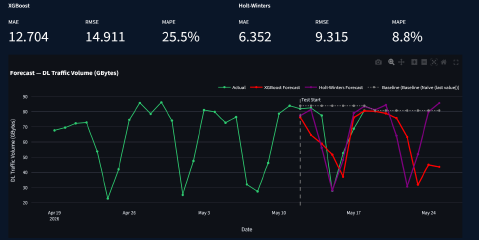
\includegraphics[width=0.95\textwidth]{figures/chapter05/image2.png}
    \caption{Forecast chart for DL Traffic Volume (GBytes) on cell \texttt{LCAIN10022-6}. The strong weekly seasonality is accurately tracked by Holt-Winters (purple), while XGBoost (red) exhibits larger deviations during the hold-out period. The naive baseline (gray dotted) flatlines at the last training value.}
    \label{fig:forecast_chart}
\end{figure}

\subsection{Residual Analysis}

For the XGBoost model, in-sample training residuals are subjected to a four-panel diagnostic suite illustrated in Figures~\ref{fig:residual_summary} and~\ref{fig:residual_diagnostics}. The diagnostic criteria are:

\begin{itemize}
    \item \textbf{Mean residual:} Should be near zero, indicating unbiased predictions.
    \item \textbf{Durbin-Watson:} Acceptable range $[1.5, 2.5]$. Values outside this interval signal autocorrelated errors.
    \item \textbf{Ljung-Box $p$-value:} Exceeding 0.05 confirms that residual autocorrelations up to lag 10 are jointly insignificant.
    \item \textbf{ACF plot:} All lags should reside within the 95\% confidence band.
    \item \textbf{Residuals vs.~fitted:} No funnel or systematic pattern should be visible, confirming homoscedasticity.
\end{itemize}

\begin{figure}[htbp]
    \centering
    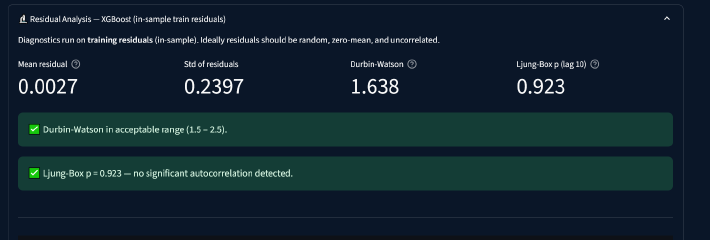
\includegraphics[width=0.95\textwidth]{figures/chapter05/image5.png}
    \caption{Residual summary statistics for XGBoost on the training set. Mean residual $=$ 0.0027, standard deviation $=$ 0.2397, Durbin-Watson $=$ 1.638 (within acceptable range), and Ljung-Box $p$-value $=$ 0.923 (no significant autocorrelation).}
    \label{fig:residual_summary}
\end{figure}

\begin{figure}[htbp]
    \centering
    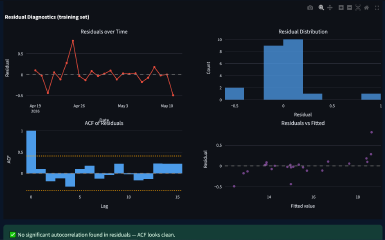
\includegraphics[width=0.95\textwidth]{figures/chapter05/image6.png}
    \caption{Four-panel residual diagnostic plot for XGBoost. Top-left: residuals over time with zero reference; top-right: residual histogram; bottom-left: ACF with 95\% confidence bands; bottom-right: residuals versus fitted values. The absence of structure supports the white-noise hypothesis.}
    \label{fig:residual_diagnostics}
\end{figure}

\subsection{Feature Importance Interpretation}

Gain-based feature importance from XGBoost reveals which engineered signals drive predictions. Figure~\ref{fig:feature_importance} displays the top-15 features for the DL Traffic Volume example. The dominance of \texttt{lag7\_norm} and \texttt{lag\_14} confirms that weekly seasonality is the primary predictive signal, while \texttt{momentum\_1} and cross-KPI features such as \texttt{Inter\_HO\_SR} capture secondary dynamics. This interpretability is operationally valuable: if a degradation in handover success rate consistently appears as a top feature for throughput forecasting, it suggests a causal coupling that network engineers can investigate.

\begin{figure}[htbp]
    \centering
    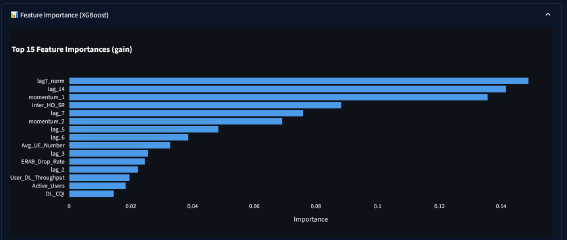
\includegraphics[width=0.95\textwidth]{figures/chapter05/image4.png}
    \caption{Top-15 XGBoost feature importance by gain for DL Traffic Volume forecasting. \texttt{lag7\_norm} and \texttt{lag\_14} dominate, confirming strong weekly periodicity. Cross-KPI features (\texttt{Inter\_HO\_SR}, \texttt{Avg\_UE\_Number}) and momentum terms contribute non-linear explanatory power.}
    \label{fig:feature_importance}
\end{figure}

Figure~\ref{fig:hyperparameters} shows the sidebar control panel through which operators adjust XGBoost hyperparameters. The conservative defaults (low \texttt{max\_depth}, moderate \texttt{learning\_rate}, subsampling) reflect the small-data regime and can be tuned per cell based on residual diagnostics.

\begin{figure}[htbp]
    \centering
    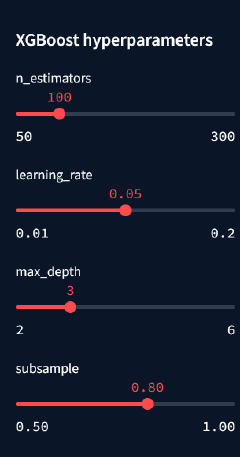
\includegraphics[width=0.45\textwidth]{figures/chapter05/image7.png}
    \caption{Streamlit sidebar exposing XGBoost hyperparameters: \texttt{n\_estimators}=100, \texttt{learning\_rate}=0.05, \texttt{max\_depth}=3, and \texttt{subsample}=0.80.}
    \label{fig:hyperparameters}
\end{figure}


\section{Chapter Summary}
\label{sec:forecasting_summary}

This chapter presented the KPI Forecasting \& Predictive Analytics Module, a multi-model engine for cell-level LTE KPI prediction. The key contributions and findings are:

\begin{itemize}
    \item A \textbf{leakage-safe feature engineering pipeline} was designed, incorporating lag features, rolling statistics, normalized shape descriptors, and cross-KPI covariates to encode temporal structure for gradient-boosted regression.

    \item \textbf{Three modeling tiers}---naive baselines, Holt-Winters exponential smoothing, and XGBoost---were implemented and evaluated under a unified protocol. An automatic fallback mechanism prevents over-reliance on complex models when simple baselines suffice.

    \item \textbf{Seasonality detection} via STL decomposition quantifies weekly pattern strength per cell-KPI pair, informing both UI ranking and model-selection expectations.

    \item \textbf{Residual diagnostics} (Durbin-Watson, Ljung-Box, ACF) confirmed that the XGBoost model captures the majority of systematic signal, leaving approximately white-noise residuals on the training set.

    \item The module exposes its outputs through an interactive Streamlit dashboard and generates \textbf{LLM-ready reports} for downstream natural-language reasoning, bridging quantitative forecasting with qualitative network optimization.
\end{itemize}
Write the chapter here.